\section{Introduction}
\label{Introduction}

This article reports on scientific discussions and conclusions elaborated at a workshop on \gls{hep} held in November 2022 at CERN in Geneva.
This first event of the Quantum Computing for HEP (QC4HEP) Working Group gathered experts on \gls{hep} from different academic and research institutions and countries over four continents, who besides being world experts in theoretical and experimental aspects of \gls{hep}, also shared a common interest in \gls{qc} and its potential as a game changer in the field. 
The main goal of the workshop, and of this report-article, is to set a common roadmap for selected topics of interest to this community, in which we believe that \gls{qc} can have a significant impact in the near future. 
To this end, we have investigated classes of problems and corresponding quantum algorithms that can lead to potential quantum advantage with near-term, noisy, quantum devices, and - in particular - using IBM superconducting devices. We aim at delivering a set of physically relevant use cases that can become interesting %playground for the 
demonstrations in view of the $100 \otimes 100$ challenge announced by IBM~\cite{IBM_100by100}. 

For practical purposes, we have organized this article into two main domain areas: theoretical methods and algorithms for modelling \gls{hep} problems, and numerical methods for the interpretation and analysis of experimental results as well as detector simulation and event generation. 
We strongly believe that there are important connections between the two research domains, where many of the quantum algorithms designed for the solution of problems in one field can also be transferred to the other. 

We will therefore start with a short summary of the main \gls{hep} domains in theoretical modelling and experimental physics, for which we believe there is the potential for quantum computing to play a significant role in the near-term.  


\subsection{Quantum Computing for Theoretical Modelling in \gls{hep}}

Despite the great success of classical lattice field theory (e.g., for \gls{qed} and \gls{qcd} simulations~\cite{Durr2008,Alexandrou2020}), out-of-equilibrium and real-time dynamics (e.g., of particle collisions, thermalization phenomena or dynamics after a quench), remain out of reach for euclidean path-integral Monte Carlo simulations. 
Furthermore, properties of nuclear matter at high fermionic densities, as they arise in neutron stars or at the very early universe  for example, can not be accessed through these classical simulation techniques~\cite{Fukushima2011}. The same holds true for theories with topological terms, which are relevant, e.g. in \gls{qcd} for understanding the amount of CP-violation or, in the electroweak sector, the sphaleron rate in the early universe.  
These severe limitations are rooted in the notorious \emph{sign-problem}: the highly oscillatory behaviour of the path integrals arising in real-time phenomena, in systems with a high fermionic particle density or in the presence of topological terms imply an exponentially growing sampling run-time complexity with an increasing number of lattice sites~\cite{Troyer2005}.

An alternative approach to circumvent the sign problem might be to describe lattice fields theories in the equivalent Hamiltonian formalism, instead of the path integral description based on the Lagrangian formalism~\cite{Kogut1975,Kogut1979}. 
In the Hamiltonian approach, however, the total many-particle wave function which describes a general particle state on the whole lattice must be stored throughout the simulation. 
But since the total discretized Hilbert space $\mathcal{H}$ containing these general states corresponds to a tensor product of Hilbert spaces $\mathcal{H}_j$ on a single lattice site, the required memory to store a full wave function on the lattice scales exponentially with the number of lattice sites.

In recent years, novel tensor network-based methods have been introduced to alleviate these limitations by allowing for a more compact representation of general quantum states on the lattice~\cite{Silvi2014,Dalmonte2016,Banuls2019SimulatingLG,Banuls2019,Banuls2020TNreview}. The underlying mechanism which allows Hamiltonian simulations to be performed is that only a small subspace of the complete Hilbert space describes the low energy physics of quantum field theories and \gls{tn} methods identify and focus exactly on these physically relevant subspaces. Hence, with tensor network techniques, various phenomena such as string breaking and real-time dynamics~\cite{Buyens2013,Kuehn2015,Pichler2016,Buyens2016b,Banuls2019b,Rigobello2021} or phase diagrams of both abelian and non-abelian gauge theories at finite fermionic densities~\cite{Banuls2016a,Silvi2017,Felser2019,Silvi2019} have been studied on a few hundred lattice sites at least in one space dimensional models. 

A very promising alternative to \gls{tn} are simulations on quantum computers which can represent large Hilbert spaces using qubits, its basic unit of information, where the number of required qubits merely grows linearly with the number of lattice sites. Moreover, quantum algorithms have been proposed that implement real-time dynamics with polynomial time complexity for scalar quantum field theories and \gls{qed}~\cite{Byrnes2006, Jordan2012, Mathis2020}. 
In addition, by sharing with tensor networks the Hamiltonian formulation, quantum computations completely avoid the sign problem. 
Thus, quantum computers offer a potential framework to fully overcome the limitations outlined above for the simulation of lattice gauge theories and especially their real-time dynamics~\cite{Feynman1982}. 

Indeed, various proposals for the implementation of general abelian and non-abelian \gls{lgt} on different types of quantum hardware have accumulated in the past few years, and simulations of small \gls{lgt} systems on real quantum devices have been demonstrated~\cite{Banuls2019SimulatingLG,Banuls2019,Klco2019,Atas2021,Ciavarella2021,Clemente2022a}. Examples include proposals for implementing lattice gauge theories using optical lattices~\cite{Banerjee2012,Tagliacozzo2013,Tagliacozzo2013a}, atomic and ultra-cold quantum matter~\cite{Buchler2005,Zohar2011,Zohar2012,Hauke2013,Zohar2013a,Zohar2013c,Banerjee2013,Zohar2015a,Laflamme2015,Gonzalez-Cuadra2017,Rico2018,Zache2018}, further proof-of-principle implementations on a real superconducting architecture~\cite{Klco2018,Klco2019,Atas2021,Ciavarella2021,Mazzola2021} and ultimately, \gls{1p1D} real-time and variational simulations of quantum electrodynamics on a trapped ion system~\cite{Martinez2016, Kokail2019}. A broad overview of recently proposed quantum simulators and implementation techniques for \gls{lgt} can be found in~\cite{Dalmonte2016,Banuls2019SimulatingLG,Banuls2019}. It is noteworthy that lattice gauge theories can be approached by many different physical systems and methods, each featuring its own advantages and disadvantages.

The understanding of the static and dynamical properties of \gls{3p1D} \gls{lgt}, including \gls{qed} and \gls{qcd}, is not the only target of today's theoretical particle physics. In fact, one has to consider an exciting but also demanding roadmap to reach eventually the goal of performing quantum simulations of \gls{3p1D} systems as relevant for \gls{hep}. This roadmap starts with \gls{1p1D} systems which are under active research nowadays, moving to \gls{2p1D} systems which are under consideration already now by various groups and reach \gls{3p1D} systems in the future. 

Lower dimensional systems in \gls{1p1D} and \gls{2p1D} dimensions are already very interesting. They share important and challenging problems with their higher-dimensional counterparts. One important example is the study of \gls{2p1D} \gls{qed} which shows the phenomena of asymptotic freedom and confinement. Asymptotic freedom is a feature of \gls{qcd}, i.e., the quantum field theory of the strong interaction between quarks and gluons. In the limit of high energies (small distances when natural units are used) the quarks become weakly interacting making perturbation theory well suited for theoretical predictions. On the contrary, at low energies the interaction becomes strong leading to particle confinement. Interestingly enough, there are also low dimensional \gls{lgt} for which the phenomena of confinement is known, which can help  shedding new lights on the theoretically harder \gls{qcd} confining mechanism (because of the large dimensionality and the high number of degrees of freedom).
As said above, one such model is \gls{2p1D} \gls{qed}, which is a compact $U(1)$ \gls{lgt}. As outlined in Section \ref{subsubsect_2+1QED},  we therefore propose this model in a lower dimension as a benchmark 
for exploring the potential of quantum computing in the near-term, noisy, regime. 

\subsection{Quantum Computing in \gls{hep} Experiments}
\gls{hep} experiments are characterised by the ability to probe the intricacies of particle physics in the Standard Model and beyond it, through performing measurements and analyses at the frontier between quantum theory and precision experimentation.
The statistical precision of experiments performed at elementary particles   scales is predicated on three classes of algorithms:
\begin{itemize}
    \item Detector operation algorithms allow detectors to efficiently obtain data that cleanly represents the fundamental interactions of matter. These detectors might feature very large amounts of very high dimensional data such as those found inside hadron colliders. These detectors require algorithms to sort significant signals from noise. Detector-based algorithms are also used to aid in inferring more complete features of a given measurement of very rare processes such as neutrino or expected New Physics interactions.
    \item Identification and reconstruction algorithms are an essential part of mapping the vast collection of pixel intensities, timings, and event counts to a coherent underlying physics structure in the data. These algorithms allow the segmentation of datasets into those which feature particular processes or states that are relevant to a given physics goal and therefore must be robust, efficient, and unbiased.
    \item Robust simulation and inference tools allow 
    particle physics experiments to compare large amounts of complex, highly structured data with parameterized theoretical predictions. These algorithms include the creation of simulated datasets that are used as templates in parametric statistical models, classification tools to enhance the sensitivity of a given measurement to some process, or the identification of statistically anomalous signals that might hint at sources of new physics. 
\end{itemize}
\gls{qc} 
encompasses
several defining characteristics that are of particular interest to experimental \gls{hep}: the potential for quantum speed-up in processing time, sensitivity to sources of correlations in data, and increased expressivity of quantum systems. 
Each of the three classes of algorithms mentioned above benefits from all three of these characteristics. Experiments running on high-luminosity accelerators need faster algorithms; identification and reconstruction algorithms need to capture correlations in signals; simulation and inference tools need to express and calculate functions that are classically intractable.

Within the existing data reconstruction and analysis paradigm, access to algorithms that exhibit quantum speed-ups would revolutionise the simulation of large-scale quantum systems and the processing of data from complex experimental set-ups. This would enable a new generation of precision measurements to probe deeper into the nature of the universe. Existing measurements may contain the signatures of underlying quantum correlations or other sources of new physics that are inaccessible to classical analysis techniques. Quantum algorithms that leverage these properties could potentially extract more information from a given dataset than classical algorithms. Finally, algorithms that can capture more complex aspects of \gls{hep} theory and simulation could provide estimators that are more natively aligned with the quantum mechanical nature of the Standard Model or indeed potentially uncover new physics beyond what can be explained by classical models.

Quantum computing for \gls{hep} is of particular interest due to the prospect of algorithms that can leverage the unique properties of quantum systems to achieve computational advantages. Most quantum algorithms with a promise of a super-polynomial advantage exploit the capacity of quantum computers to efficiently simulate quantum-many-body systems. The search for potential quantum advantage would be accelerated by the identification of computational problems with the right kind of underlying structure which can be leveraged by quantum algorithms. Applications in the \gls{hep} domain can clearly offer a controlled experimental benchmark for such test cases. Through the analysis of the data from \gls{hep} experiments using quantum algorithms, researchers may be able to gain insights into the behaviour of quantum systems and potentially identify new avenues for quantum advantage.

\gls{hep} experimental data is typically organized as collections of associated detector signals that can be reconstructed into measured particles. The distributions of these particle measurements are calculable under specific parameterization of the underlying theory such that the distribution of experimental data can be directly compared to theoretical predictions through the use of simulated data.
These parameterizations are such that a characterisation of any given process as defined in quantum field theory is maximally described by the data. 
This method of parameterization allows the accuracy of the estimator to scale consistently and efficiently with repeated measurements.
Therefore, although the data recorded in high-energy physics experiments provide information about the behaviour of fundamental particles and their interactions, which in turn are described by quantum fields and their dynamics governed by the principles of quantum mechanics, it is important to note that typically the data and their descriptions are classical in nature and therefore may not trivially exhibit the quantum mechanical properties necessary for quantum advantage. 
In summary, by analyzing experimental data using tools and techniques from both quantum information theory and particle physics, we can gain insights into the fundamental nature of the universe and potentially discover new phenomena that are not yet understood.

It is worth mentioning that another community article on quantum simulations for \gls{hep} appeared recently in the literature~\cite{PRXQuantum.4.027001}. 
Despite the broadly similar target, our work differentiates in several essential aspects; first, our focus is on the identification and detailed characterization of projects that - while approachable with near-term, noisy quantum devices (within the $100 \otimes 100$ challenge) -  can already address problems of interest in the \gls{hep} community. Second, our investigation comprises both theoretical models as well as computational aspects related to particle collision experiments.

\begin{figure}[htp!]
    \centering
    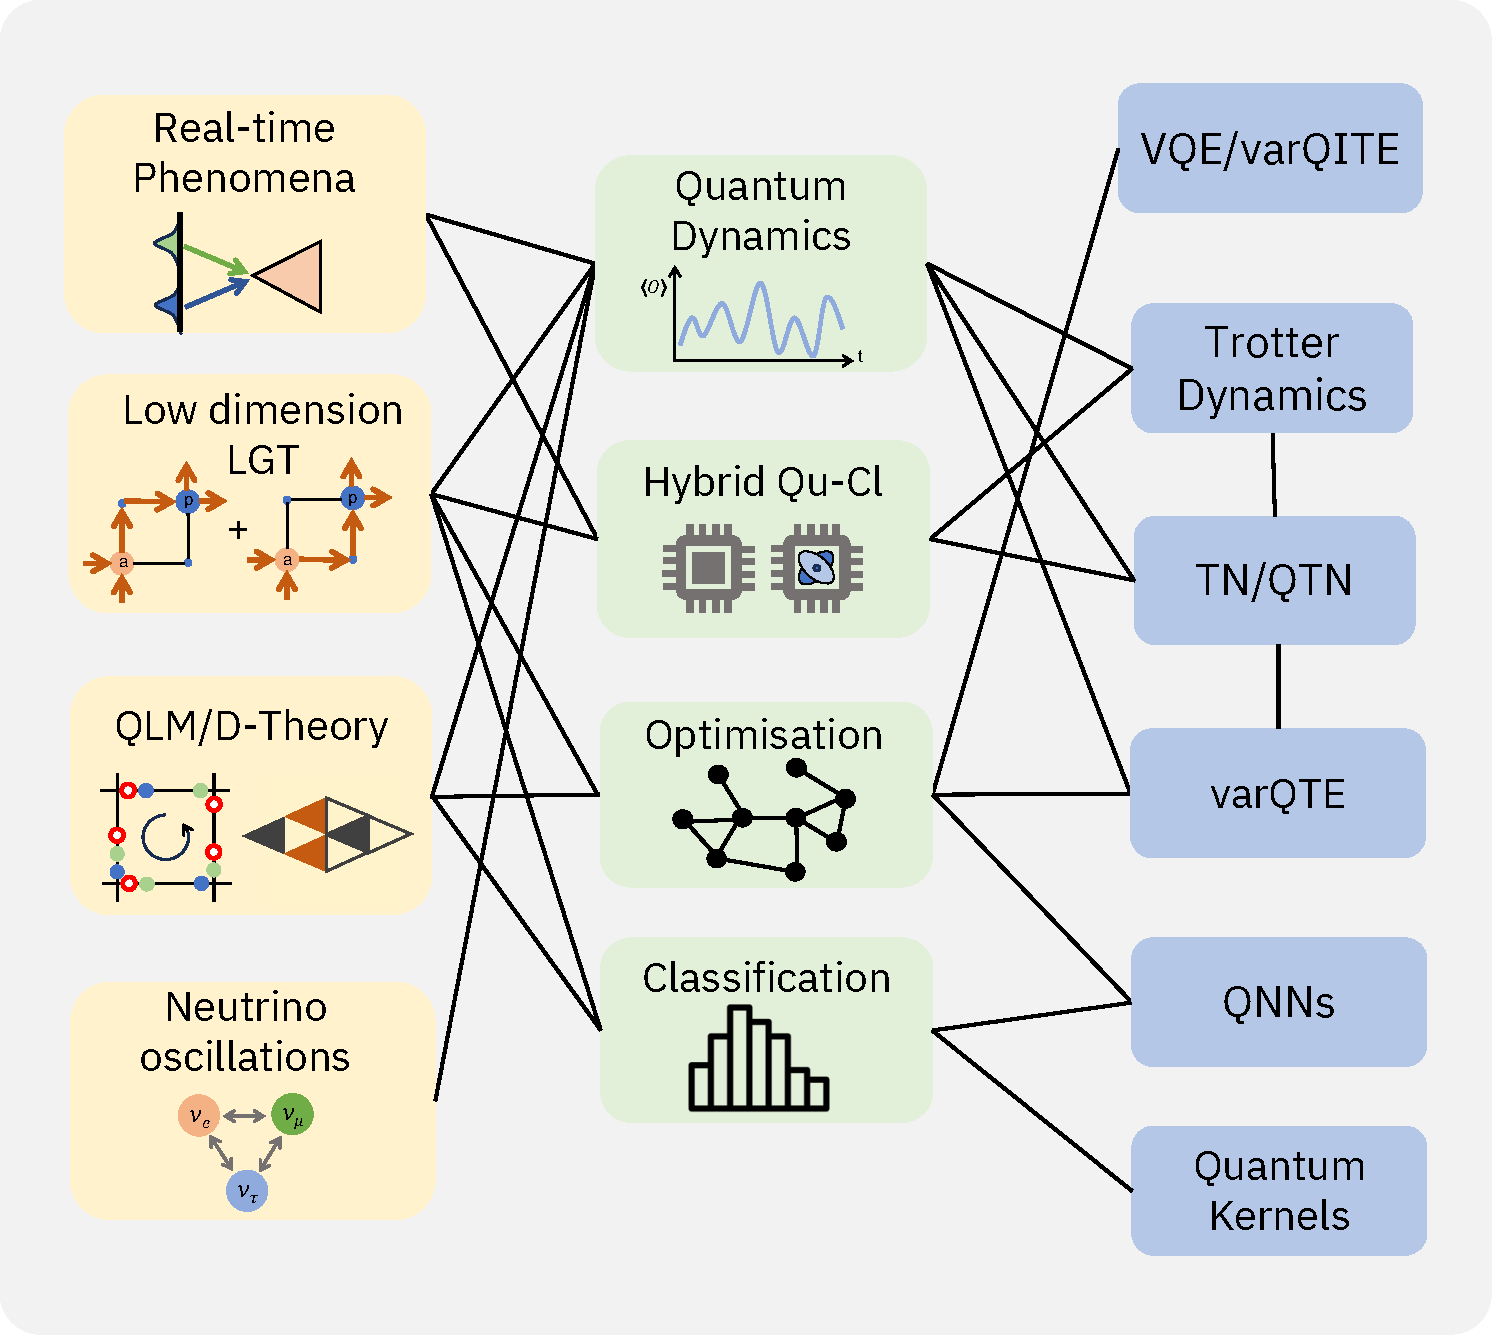
\includegraphics[width=.95 \columnwidth, keepaspectratio]{figures/Figure1a.pdf} \\
    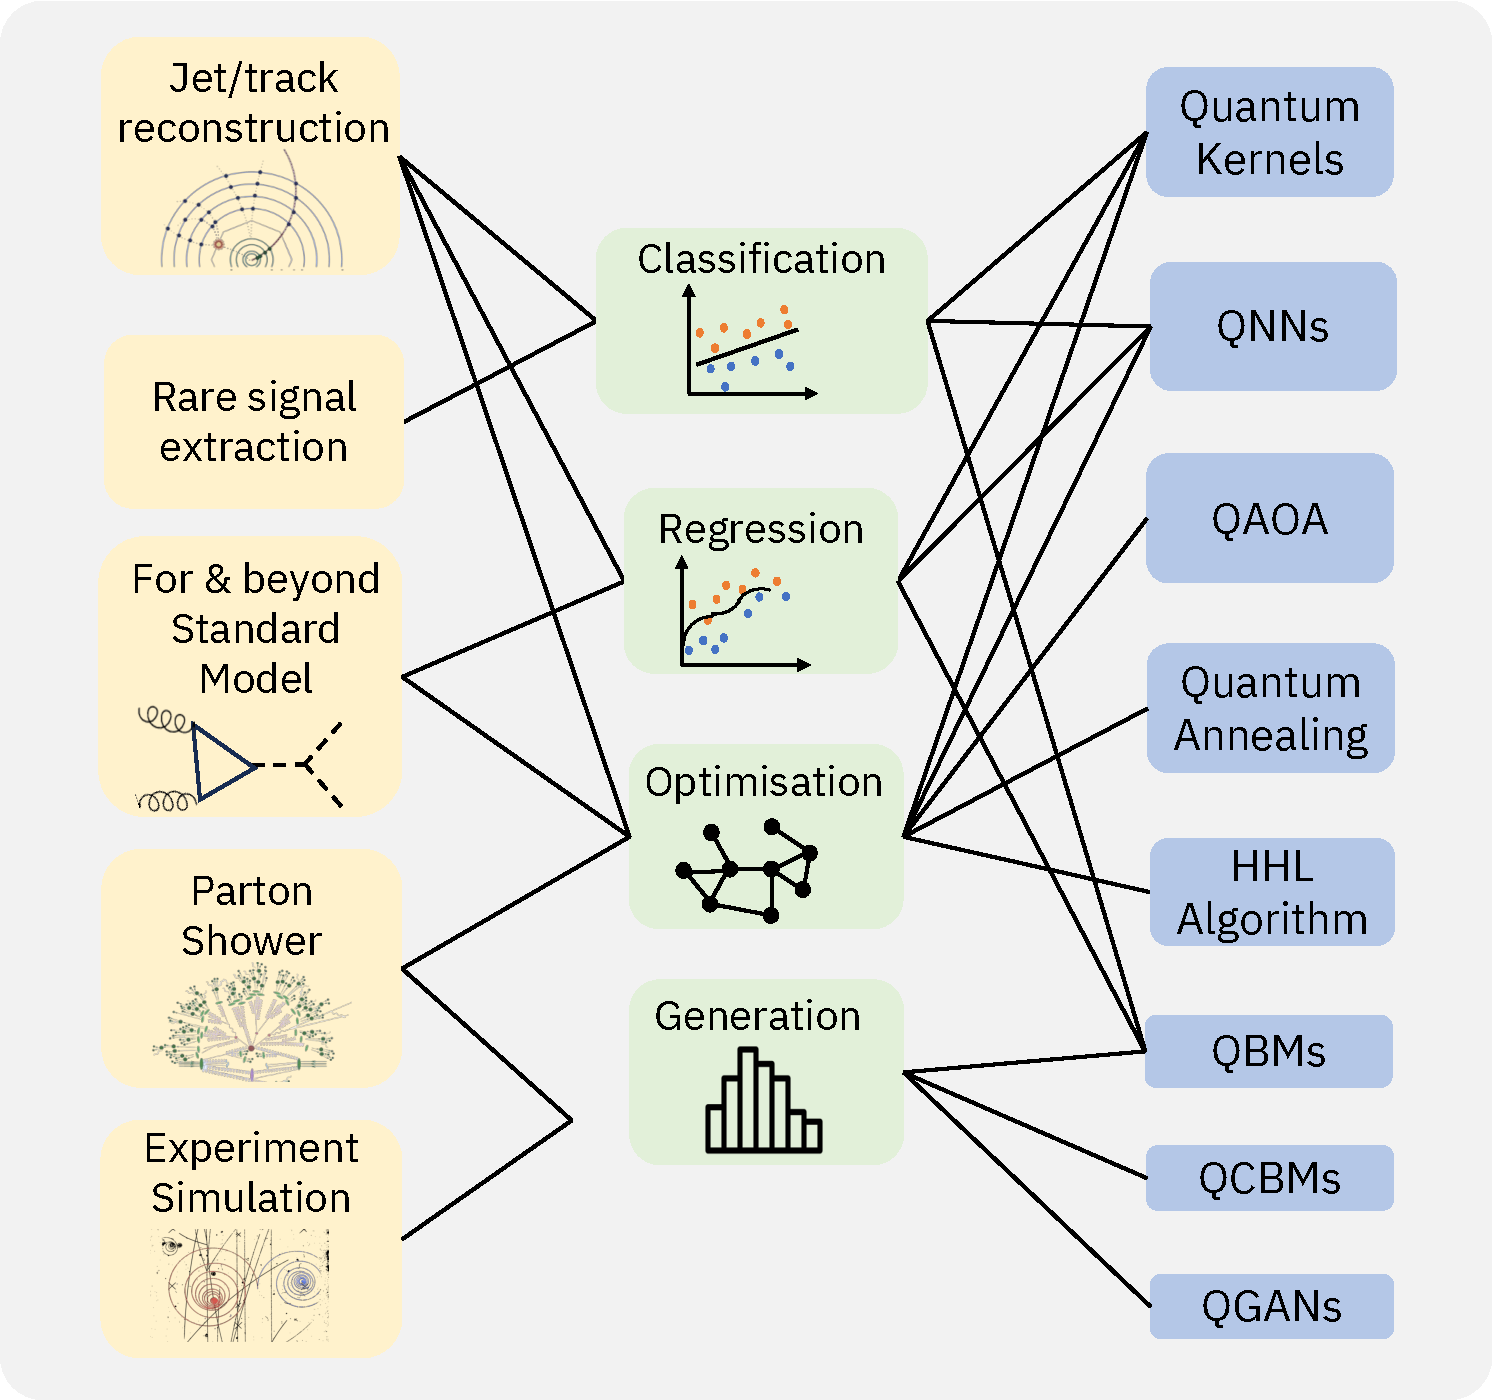
\includegraphics[width=.95 \columnwidth, keepaspectratio]{figures/Figure1b.pdf}
    \caption{(Upper Panel) Proposed theoretical physical model systems (orange) with corresponding approaches (green) and quantum algorithms (blue). For more information on the identified areas of interest see Section~\ref{subsect_Theory}. 
    (Lower Panel) 
    Proposed experimental challenges (orange) with corresponding approaches (green) and quantum algorithms (blue). For more information on the identified areas of interest see Section~\ref{subsect_Experiments}. 
    Legend: 
    VQE: Variational Eigensolver; 
    varQITE: variational Imaginary Time evolition;
    Tortter Dynamics: Time evolution based on trotteried time propagation operator;
    TN: Tensor Networks;
    QTN: Quantum Tensor Networks inspired from classical TN; 
    varQTE: variational Quantum Real Time evolution;
    QNN: Quantum Neural Networks;
    QAOA: Quantum Approximate Optimization Algorithm; 
    HHL Algorith:  Quantum algorithm for linear systems of equations (by Aram Harrow, Avinatan Hassidim, and Seth Lloyd);
    QBM: Quantum Boltzman Machines;
    QCBM: Quantum Circuit Born Machine; 
    QGANs: Quantum Generative Adversarial Networks.
    See Appendix~\ref{app:algos_limits} for an overview of a selection of these methods.}
    \label{fig:qiskit-merged}
\end{figure}


This article is organized as follows. In Sec.~\ref{sec:ibm_roadmap}, we outline IBM's roadmap for future quantum devices and explain why digital quantum computers are suitable for addressing open challenges in \gls{hep}. Subsequently we describe the challenges in the field and goals that are one hopes to achieve utilizing quantum hardware in Sec.~\ref{sec:goals}. Section~\ref{sec:algs} contains a description of various algorithms that we consider as key candidates for achieving the goals outlined in the previous section. Finally, we conclude in Sec.~\ref{sec:conclusion_outlook}. In appendix~\ref{appendix_resources}, we provide a detailed estimation of the required resources for encoding lattice gauge theories in a digital, qubit-based quantum computer, while appendix~\ref{app:algos_limits} contains information on selected quantum and classical algorithms.
